                %%%%%%%%%%%%%%%%%%%%%%%%%%%%%%%%%%%%%%%%%
% Beamer Presentation
% LaTeX Template
% Version 1.0 (10/11/12)
%
% This template has been downloaded from:
% http://www.LaTeXTemplates.com
%
% License:
% CC BY-NC-SA 3.0 (http://creativecommons.org/licenses/by-nc-sa/3.0/)
%
%%%%%%%%%%%%%%%%%%%%%%%%%%%%%%%%%%%%%%%%%

%----------------------------------------------------------------------------------------
%   PACKAGES AND THEMES
%----------------------------------------------------------------------------------------

\documentclass{beamer}

\mode<presentation> {

% The Beamer class comes with a number of default slide themes
% which change the colors and layouts of slides. Below this is a list
% of all the themes, uncomment each in turn to see what they look like.

%\usetheme{default}
%\usetheme{AnnArbor}
%\usetheme{Antibes}
%\usetheme{Bergen}
%\usetheme{Berkeley}
%\usetheme{Berlin}
%\usetheme{Boadilla}
%\usetheme{CambridgeUS}
%\usetheme{Copenhagen}
%\usetheme{Darmstadt}
%\usetheme{Dresden}
%\usetheme{Frankfurt}
%\usetheme{Goettingen}
%\usetheme{Hannover}
%\usetheme{Ilmenau}
%\usetheme{JuanLesPins}
%\usetheme{Luebeck}
\usetheme{Madrid}
%\usetheme{Malmoe}
%\usetheme{Marburg}
%\usetheme{Montpellier}
%\usetheme{PaloAlto}
%\usetheme{Pittsburgh}
%\usetheme{Rochester}
%\usetheme{Singapore}
%\usetheme{Szeged}
%\usetheme{Warsaw}

% As well as themes, the Beamer class has a number of color themes
% for any slide theme. Uncomment each of these in turn to see how it
% changes the colors of your current slide theme.

%\usecolortheme{albatross}
%\usecolortheme{beaver}
%\usecolortheme{beetle}
%\usecolortheme{crane}
%\usecolortheme{dolphin}
%\usecolortheme{dove}
%\usecolortheme{fly}
%\usecolortheme{lily}
%\usecolortheme{orchid}
%\usecolortheme{rose}
%\usecolortheme{seagull}
%\usecolortheme{seahorse}
%\usecolortheme{whale}
%\usecolortheme{wolverine}

%\setbeamertemplate{footline} % To remove the footer line in all slides uncomment this line
%\setbeamertemplate{footline}[page number] % To replace the footer line in all slides with a simple slide count uncomment this line

%\setbeamertemplate{navigation symbols}{} % To remove the navigation symbols from the bottom of all slides uncomment this line
}
\usepackage[italian]{babel}
\usepackage[utf8]{inputenc}
\usepackage{graphicx} % Allows including images
\usepackage{booktabs} % Allows the use of \toprule, \midrule and \bottomrule in tables


%----------------------------------------------------------------------------------------
%   TITLE PAGE - TITLE SLIDE 1
%----------------------------------------------------------------------------------------

\title[Device-To-Device Smart Parking]{Progettazione ed implementazione di un sistema \\Smart Parking basato su comunicazione Device-To-Device}

\author{Presentata da: \\Andrea Sghedoni} % Your name
\institute[]{Alma Mater Studiorum $\cdot$ Universit\`a di Bologna \\ SCUOLA DI SCIENZE \\ Corso di Laurea Magistrale in Informatica}
\date[16/03/2016]{Sessione III \\ Anno Accademico 2015/2016} % Date, can be changed to a custom date

\begin{document}
\begin{frame}
\maketitle
\textbf{Relatore:} Chiar.mo Prof. Marco Di Felice\\
\textbf{Correlatore:} Dott. Federico Montori
\end{frame}

%----------------------------------------------------------------------------------------
%   INDEX PRESENTATION SLIDE 2
%----------------------------------------------------------------------------------------

\begin{frame}
\frametitle{Indice}
\begin{itemize}
  \item Il parcheggio
  \item Il Crowdsensing
  \item Simulazione e Modellazione
  \item Risultati
  \item Conclusioni
\end{itemize}
\end{frame}


%----------------------------------------------------------------------------------------
%   PARCHEGGIO PRESENTATION SLIDE 3
%----------------------------------------------------------------------------------------
\begin{frame}
\frametitle{Il parcheggio}
\begin{itemize}
  \item Il continuo processo di urbanizzazione ha portato sovraffollamento di autoveicoli nelle città metropolitane
  \item Più del 30\% della congestione del traffico è causata da utenti in cerca di parcheggio
  \item Parcheggi on-street
  \item Conseguenze negative:
    \begin{itemize}
      \item perdita di tempo e denaro
      \item inquinamento ambientale (CO\ped{2})
      \item peggioramento della qualità di vita
    \end{itemize}
\end{itemize}
\end{frame}


%----------------------------------------------------------------------------------------
%   CROWDSENSING PRESENTATION SLIDE 4
%----------------------------------------------------------------------------------------
\begin{frame}
\frametitle{Il Crowdsensing}
\begin{itemize}
  \item Condivisione di dati con la collettività
  \item Intelligenza condivisa
  \item Il singolo contribuisce al benessere collettivo
\end{itemize}
\end{frame}


%----------------------------------------------------------------------------------------
%   SCENARIO GENERALE E RUOLI UTENTE SLIDE 5
%----------------------------------------------------------------------------------------
\begin{frame}
\frametitle{Architettura IoE}
\begin{columns}
\begin{column}{0.4\textwidth}
\begin{itemize}
  \item Città metropolitana
  \item Alta dinamicità
  \item Ruoli dei device:
    \begin{itemize}
    \item Access Point
    \item client
  \end{itemize}
\end{itemize}
\end{column}

\begin{column}{0.4\textwidth}
\begin{figure}
\raggedleft
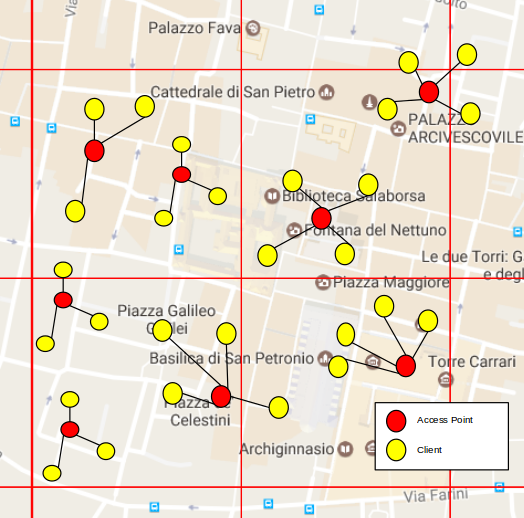
\includegraphics[width=\columnwidth]{img/arch_general.png}
\end{figure}
\end{column}
\end{columns}
\end{frame}


%----------------------------------------------------------------------------------------
%   ARCH. SOFTWARE E RUOLI UTENTE SLIDE 6
%----------------------------------------------------------------------------------------
\begin{frame}
\frametitle{Architettura IoE}
\begin{figure}
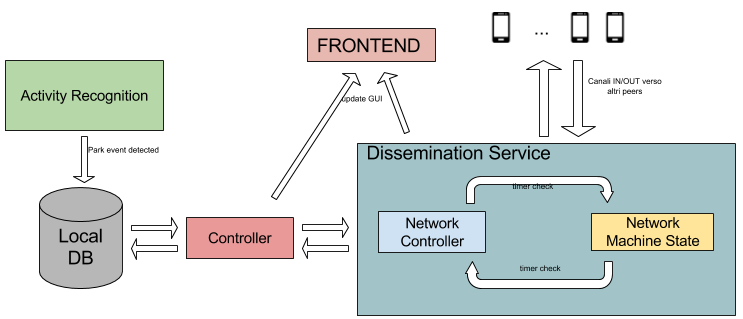
\includegraphics[scale=0.25]{img/arch_soft.png}
\end{figure}
\end{frame}


%----------------------------------------------------------------------------------------
%   PROBABILITA - SLIDE X
%----------------------------------------------------------------------------------------
\begin{frame}
\frametitle{Probabilità di parcheggio}

\begin{itemize}
  \item Sincronizzazione sugli eventi parcheggio/rilascio della cella \textit{i}
  \item Eventi parcheggio $E\ped{i}\ap{p}$ e rilascio $E\ped{i}\ap{r}$
  \item Slot totali $N\ped{i}\ap{t}$ noto a priori
  \item Slot occupati:
  \\
  {\centering $N\ped{i}\ap{o} = E\ped{i}\ap{p} - E\ped{i}\ap{r}$\par}
  \vspace{2mm}
  \item Tasso di occupazione:
  \\
  {\centering $p\ped{i}\ap{o} = \frac{N\ped{i}\ap{o}}{N\ped{i}\ap{t}}$\par}
  \vspace{2mm}
  \item Probabilità di trovare parcheggio:
  \\
  \vspace{4mm}
  \centering \framebox{$p\ped{i}\ap{f} = 1 - p\ped{i}\ap{o}$}
\end{itemize}
\end{frame}


%----------------------------------------------------------------------------------------
%   SIMULAZIONE - SLIDE X
%----------------------------------------------------------------------------------------
\begin{frame}
\frametitle{Simulazione e Modellazione}
\begin{columns}
  \begin{column}{0.65\textwidth}
    \begin{itemize}
      \item OMNeT++, Veins, SUMO
      \item Zona nord-est di Bologna 1.5km x 2.5km
      \item Verificare l’efficacia del processo di spreading
      \item circa 3000 veicoli in 1800 simsec
      \item Modulo \textit{SmartParking} per modellazione logica
      \item Tecnologie considerate : 
	\begin{itemize}
	  \item V2V \textit{802.11p}
	  \item D2D \textit{WiFi Direct} 
	  \item \textit{Bluetooth}
	\end{itemize}
    \end{itemize}
  \end{column}

  \begin{column}{0.35\textwidth}
    \begin{figure}
    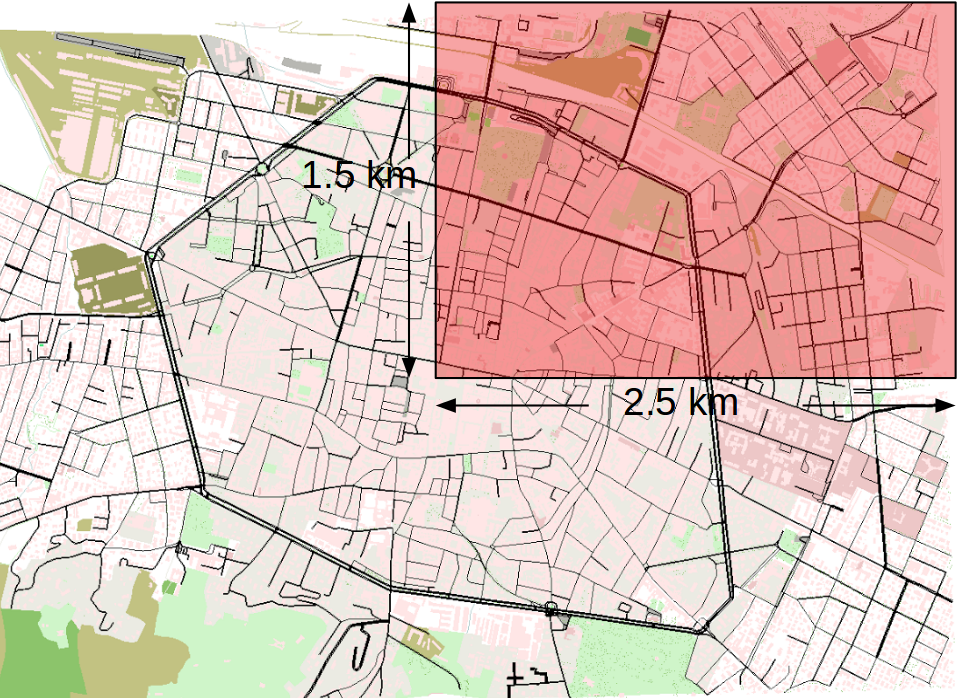
\includegraphics[width=\columnwidth]{img/sumo-bolo2.png}
    \end{figure}
  \end{column}
\end{columns}
\end{frame}


%----------------------------------------------------------------------------------------
%   RISULTATI 1 - SLIDE X
%----------------------------------------------------------------------------------------
\begin{frame}
\frametitle{Risultati (1)}
\begin{itemize}
  \item convergenza sulla conoscenza della cella corrente e dello scenario generale
\end{itemize}
\begin{columns}
  \begin{column}{0.45\textwidth}
    \begin{figure}
    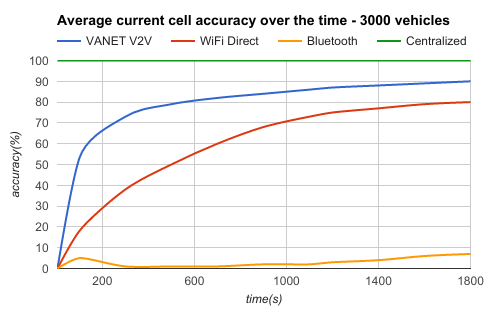
\includegraphics[width=\columnwidth]{img/graphics/local_accuracy.png}
    \end{figure}
    
  \end{column}
  \begin{column}{0.45\textwidth}
    \begin{figure}
    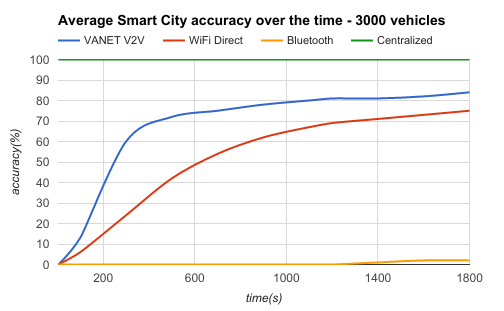
\includegraphics[width=\columnwidth]{img/graphics/global_accuracy.png}
    \end{figure}
  \end{column}
\end{columns}
\end{frame}


%----------------------------------------------------------------------------------------
%   RISULTATI 2 - SLIDE X
%----------------------------------------------------------------------------------------
\begin{frame}[shrink=50]
\frametitle{Risultati (2)}
\begin{columns}
  \begin{column}{0.45\textwidth}
    \vspace{30mm}
    \begin{figure}
    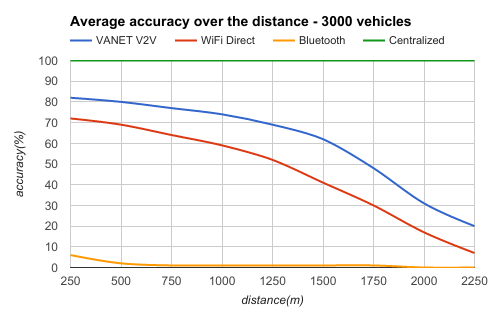
\includegraphics[width=\columnwidth]{img/graphics/distance.png}
    \end{figure}
    \begin{itemize}
      \item  L'accuratezza media decresce all'aumentare della distanza dalla posizione corrente
      \item  L'accuratezza migliore nel raggio di 500m della posizione corrente (sincronizzazioni su cella corrente e adiacenti)
    \end{itemize}
  \end{column}
  \begin{column}{0.45\textwidth}
    \vspace{20mm}
    \begin{figure}
    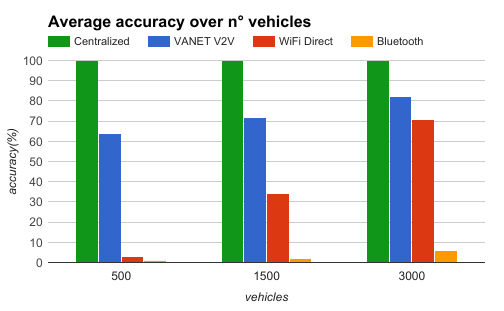
\includegraphics[width=\columnwidth]{img/graphics/n_car.png}
    \end{figure}
    \begin{itemize}
      \item  Tasso di partecipazione determinante per la tecnologia D2D \textit{WiFi Direct}
    \end{itemize}
  \end{column}
\end{columns}
\end{frame}

%----------------------------------------------------------------------------------------
%   SCREENSHOT 1 - SLIDE X
%----------------------------------------------------------------------------------------
% \begin{frame}
% \frametitle{Screenshot 1}
% \begin{columns}
%   \begin{column}{0.3\textwidth}
%     \begin{figure}
%     \raggedleft
%     \setlength{\fboxsep}{0pt}
%     \setlength{\fboxrule}{0.1pt}
%     \fcolorbox{blue}{blue}{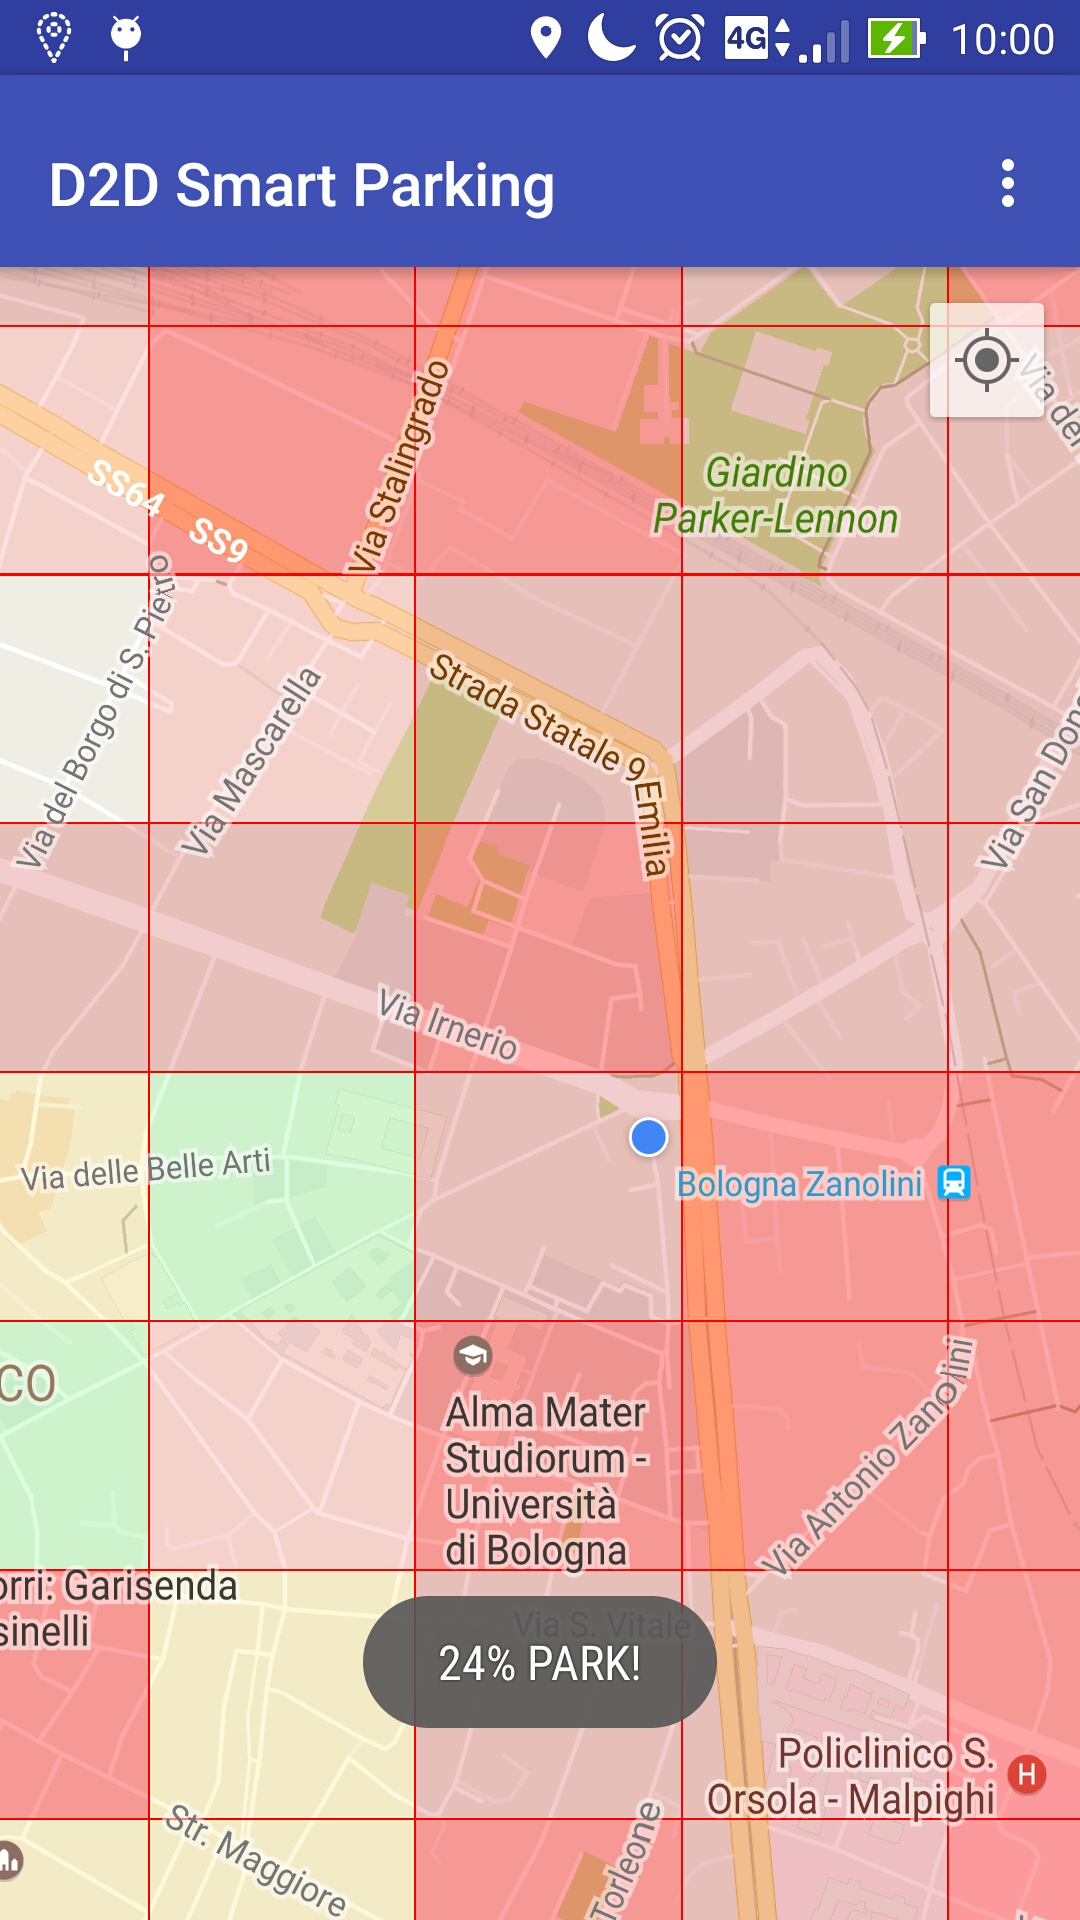
\includegraphics[width=\columnwidth]{img/screenshot/map2.jpg}}
%     \end{figure}
%   \end{column}
%   \begin{column}{0.3\textwidth}
%     \begin{figure}
%     \raggedleft
%     \setlength{\fboxsep}{0pt}
%     \setlength{\fboxrule}{0.1pt}
%     \fcolorbox{blue}{blue}{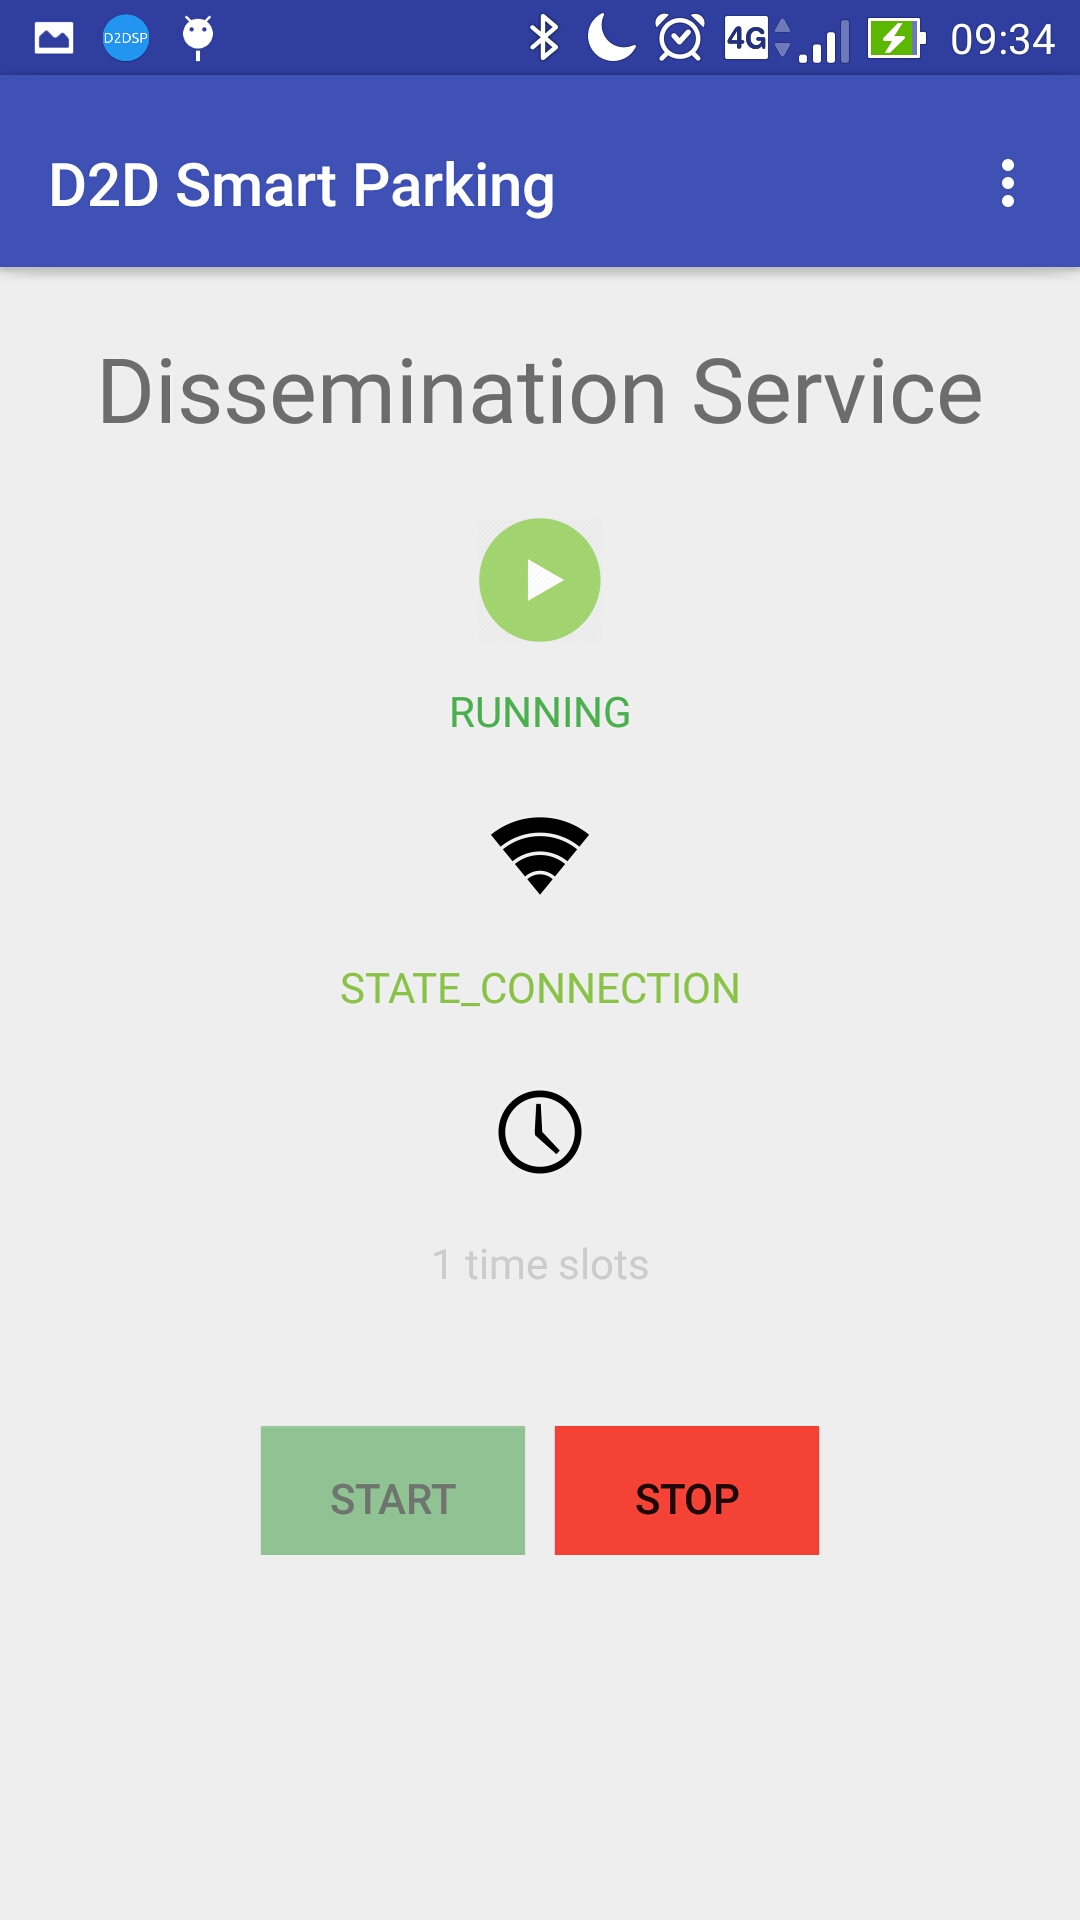
\includegraphics[width=\columnwidth]{img/screenshot/state_conn.jpg}}
%     \end{figure}
%   \end{column}
%   \begin{column}{0.3\textwidth}
%     \begin{figure}
%     \raggedleft
%     \setlength{\fboxsep}{0pt}
%     \setlength{\fboxrule}{0.1pt}
%     \fcolorbox{blue}{blue}{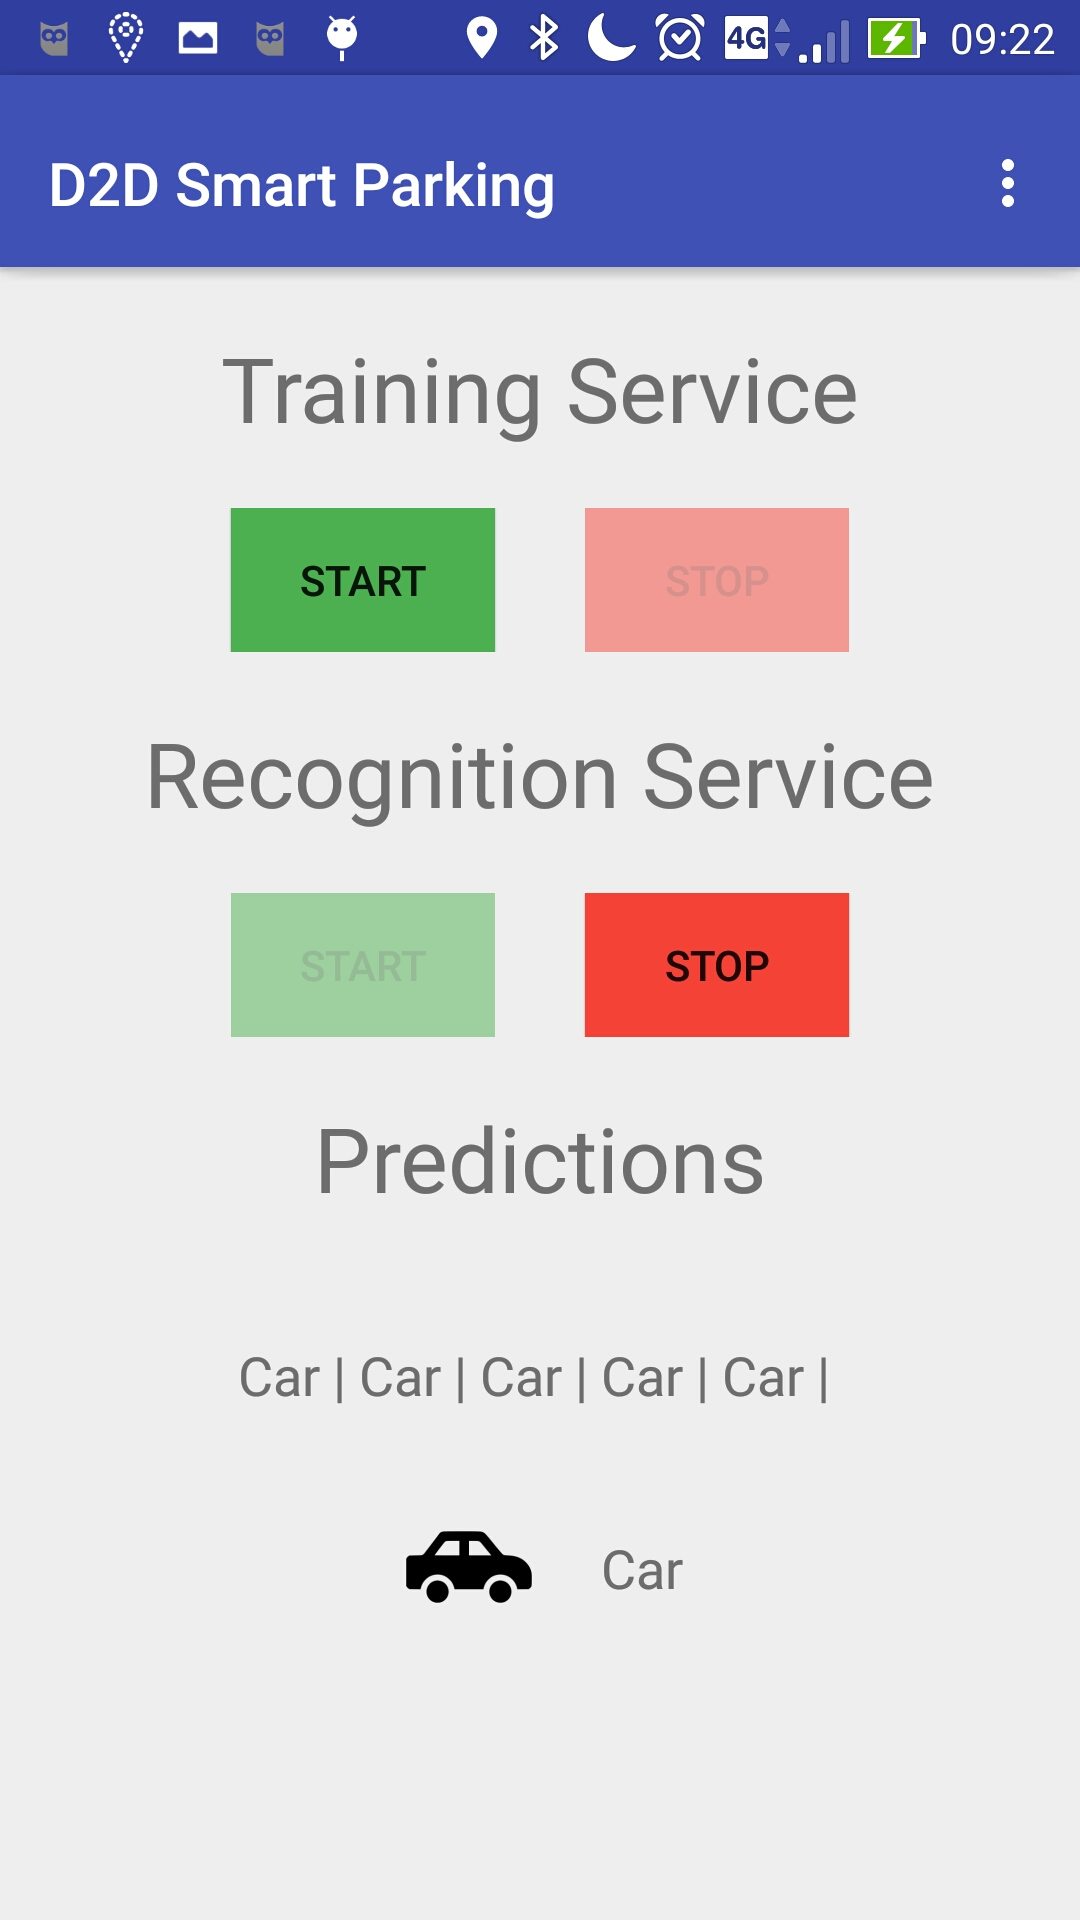
\includegraphics[width=\columnwidth]{img/screenshot/activity_recogn.jpg}}
%     \end{figure}
%   \end{column}
% \end{columns}
% \end{frame}


%----------------------------------------------------------------------------------------
%   SCREENSHOT 2 - SLIDE X
%----------------------------------------------------------------------------------------
% \begin{frame}
% \frametitle{Screenshot 2}
% \begin{columns}
%   \begin{column}{0.1\textwidth}
%   \end{column}
%   \begin{column}{0.3\textwidth}
%     \begin{figure}
%     \raggedleft
%     \setlength{\fboxsep}{0pt}
%     \setlength{\fboxrule}{0.1pt}
%     \fcolorbox{blue}{blue}{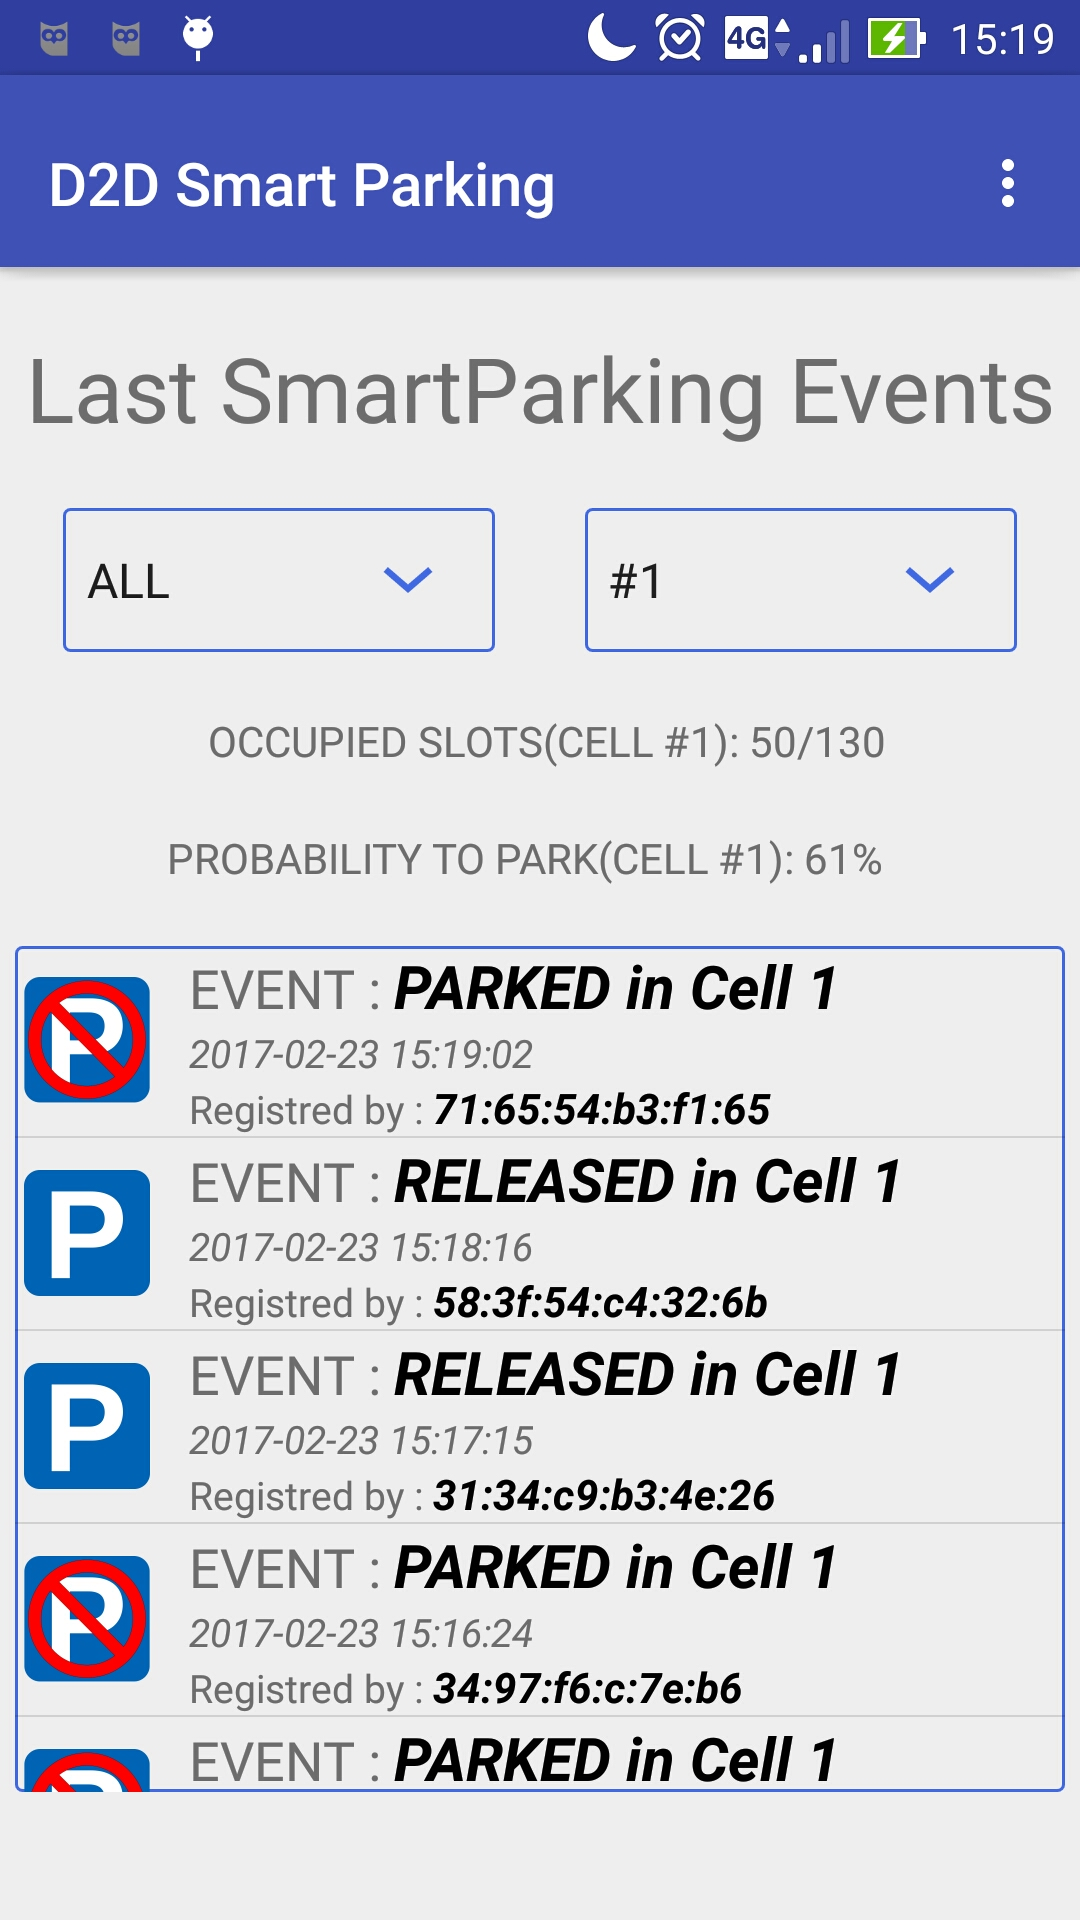
\includegraphics[width=\columnwidth]{img/screenshot/park_event_list.jpg}}
%     \end{figure}
%   \end{column}
%   \begin{column}{0.3\textwidth}
%     \begin{figure}
%     \raggedleft
%     \setlength{\fboxsep}{0pt}
%     \setlength{\fboxrule}{0.1pt}
%     \fcolorbox{blue}{blue}{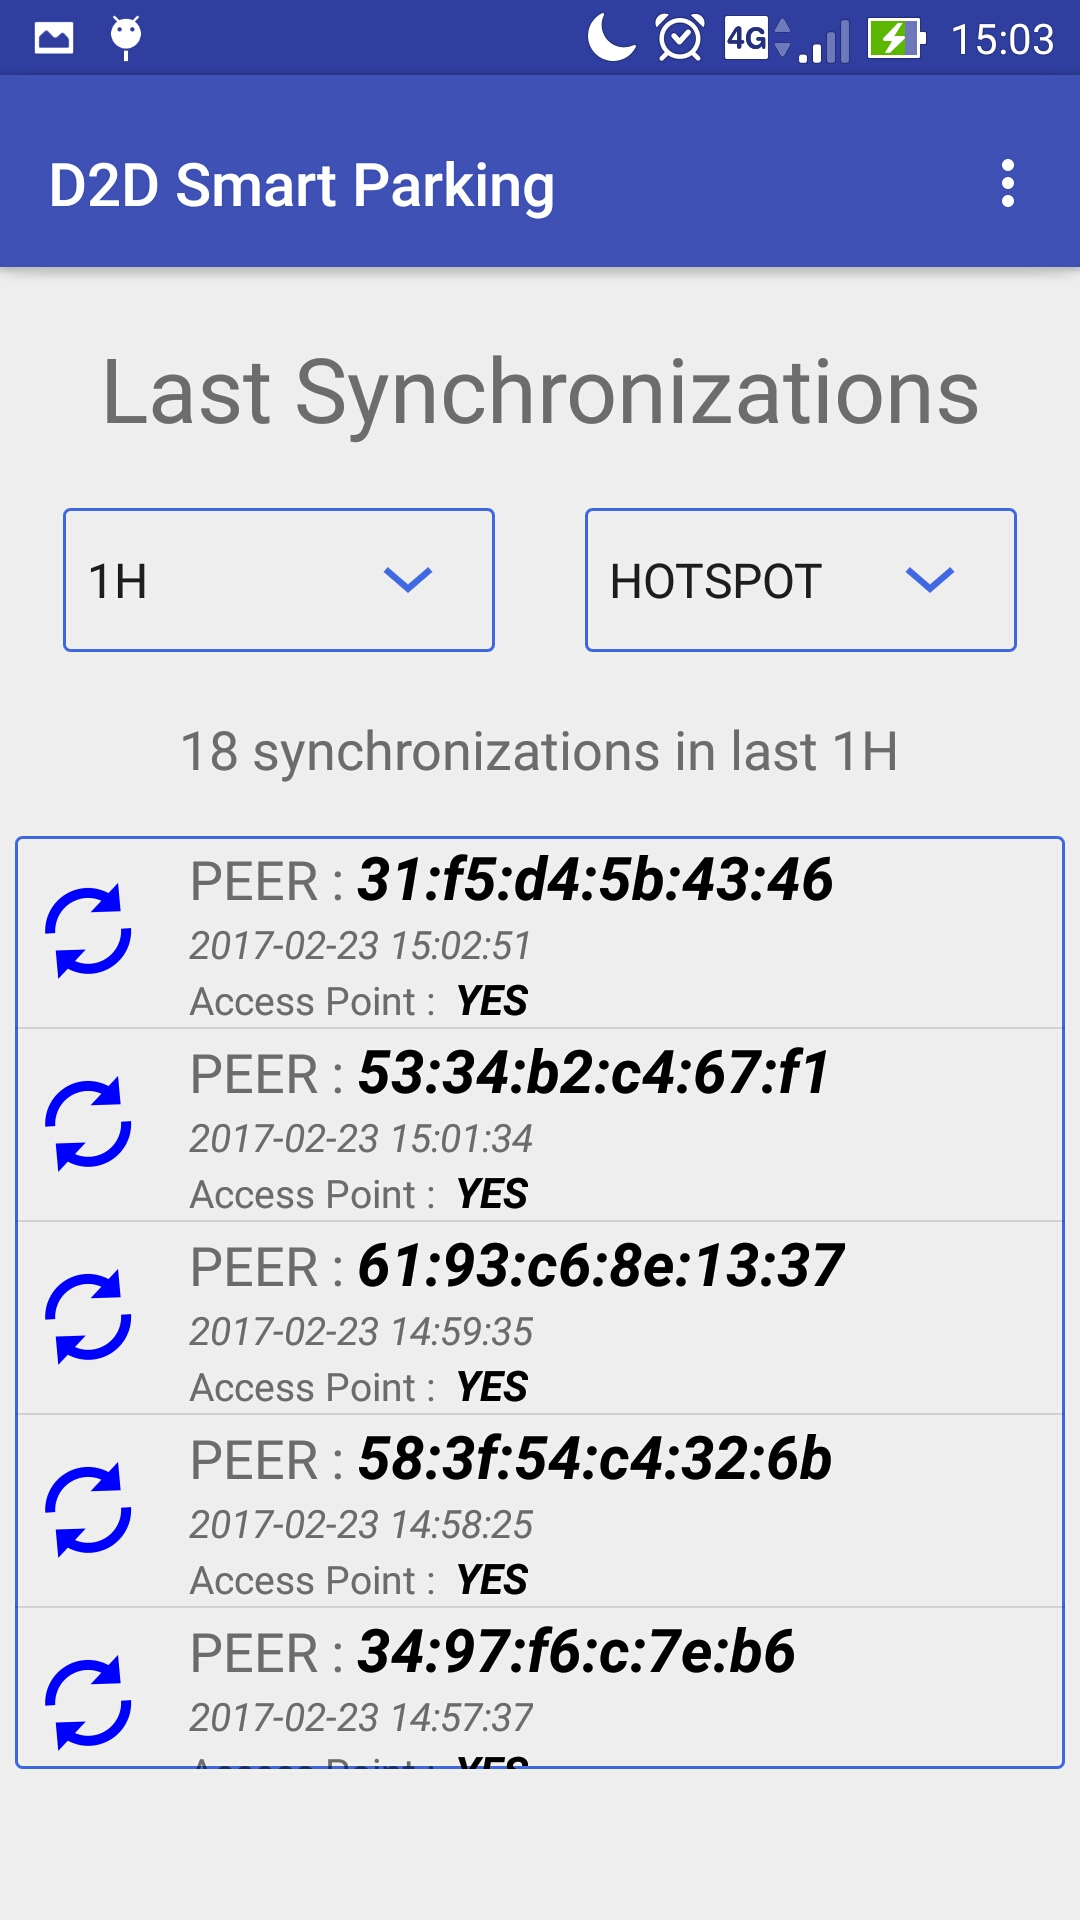
\includegraphics[width=\columnwidth]{img/screenshot/last_sync.jpg}}
%     \end{figure}
%   \end{column}
%   \begin{column}{0.1\textwidth}
%   \end{column}
% \end{columns}
% \end{frame}


%----------------------------------------------------------------------------------------
%   SCREENSHOT 1 - SLIDE X
%----------------------------------------------------------------------------------------
\begin{frame}
\frametitle{Screenshot 1}
\begin{columns}
  \begin{column}{0.25\textwidth}
    \begin{figure}
    \raggedleft
    \setlength{\fboxsep}{0pt}
    \setlength{\fboxrule}{0.1pt}
    \fcolorbox{blue}{blue}{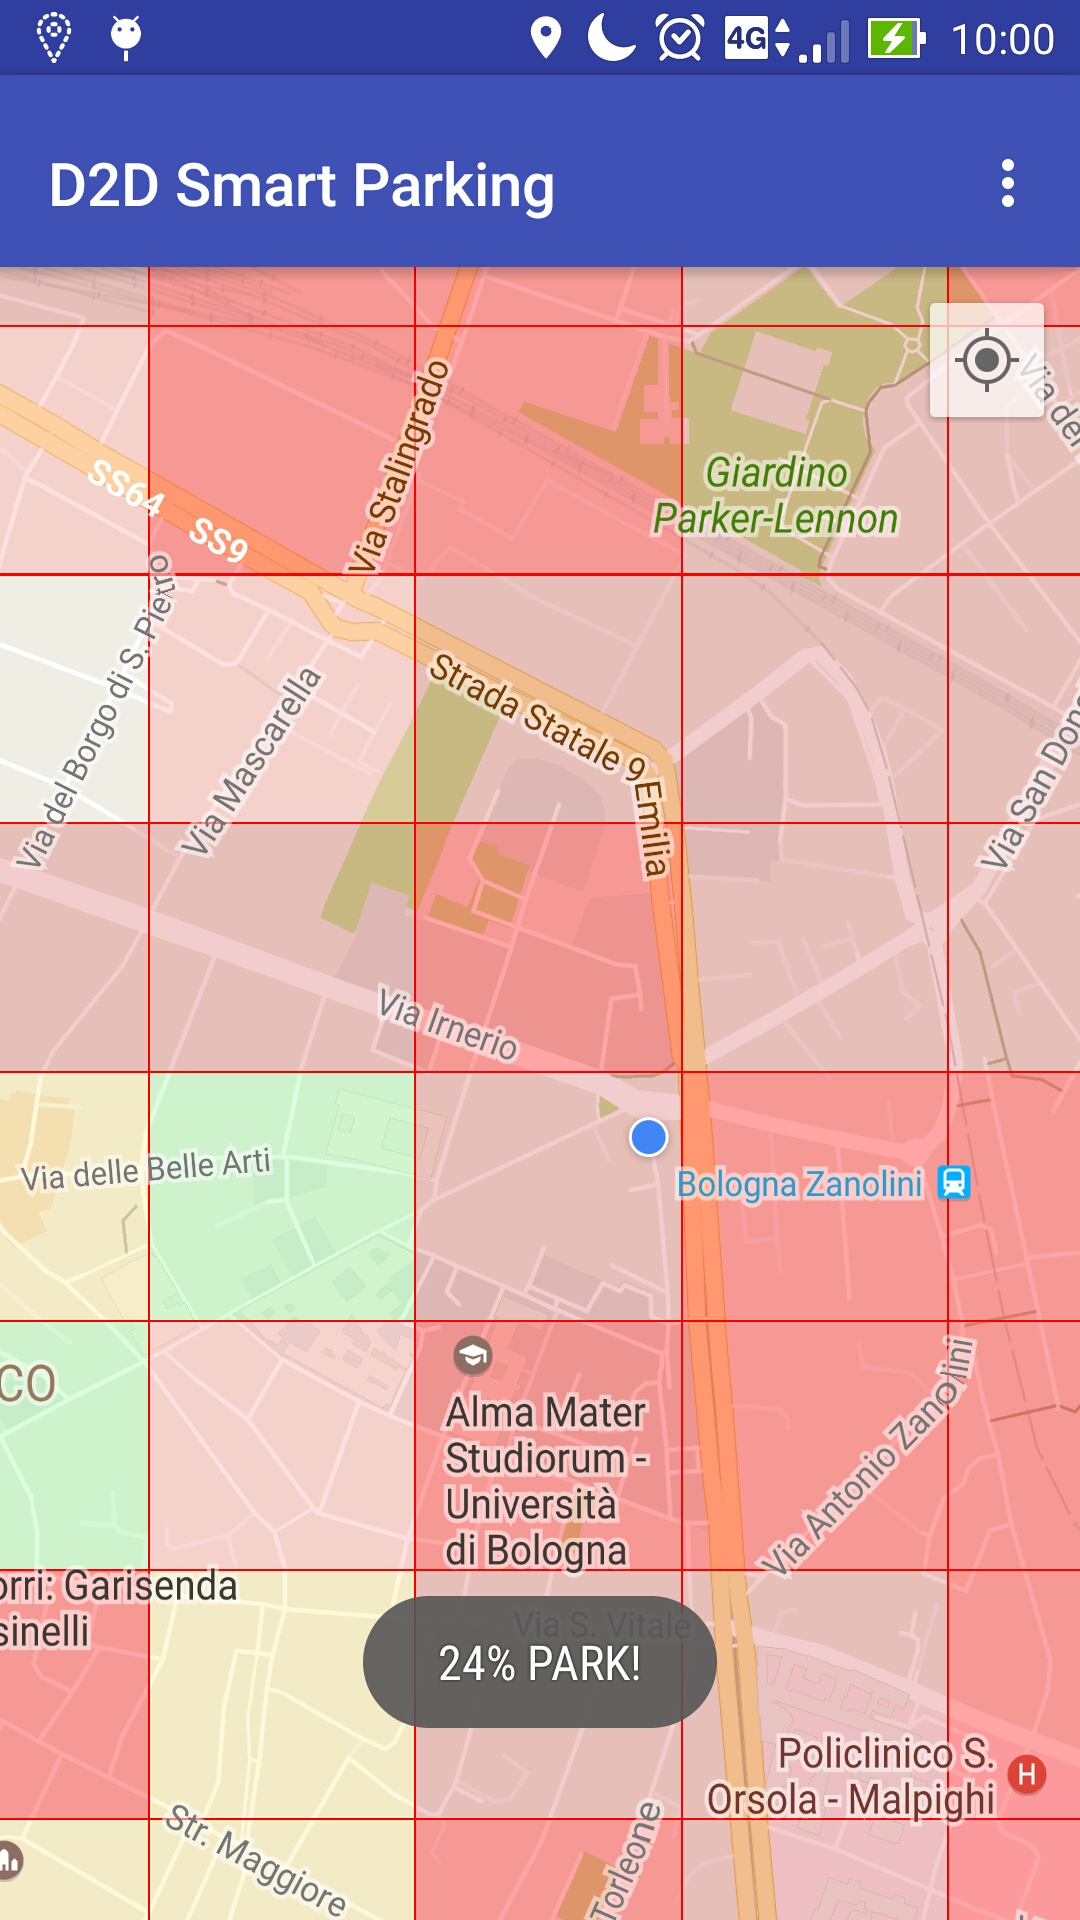
\includegraphics[width=\columnwidth]{img/screenshot/map2.jpg}}
    \end{figure}
  \end{column}
  \begin{column}{0.25\textwidth}
    \begin{figure}
    \raggedleft
    \setlength{\fboxsep}{0pt}
    \setlength{\fboxrule}{0.1pt}
    \fcolorbox{blue}{blue}{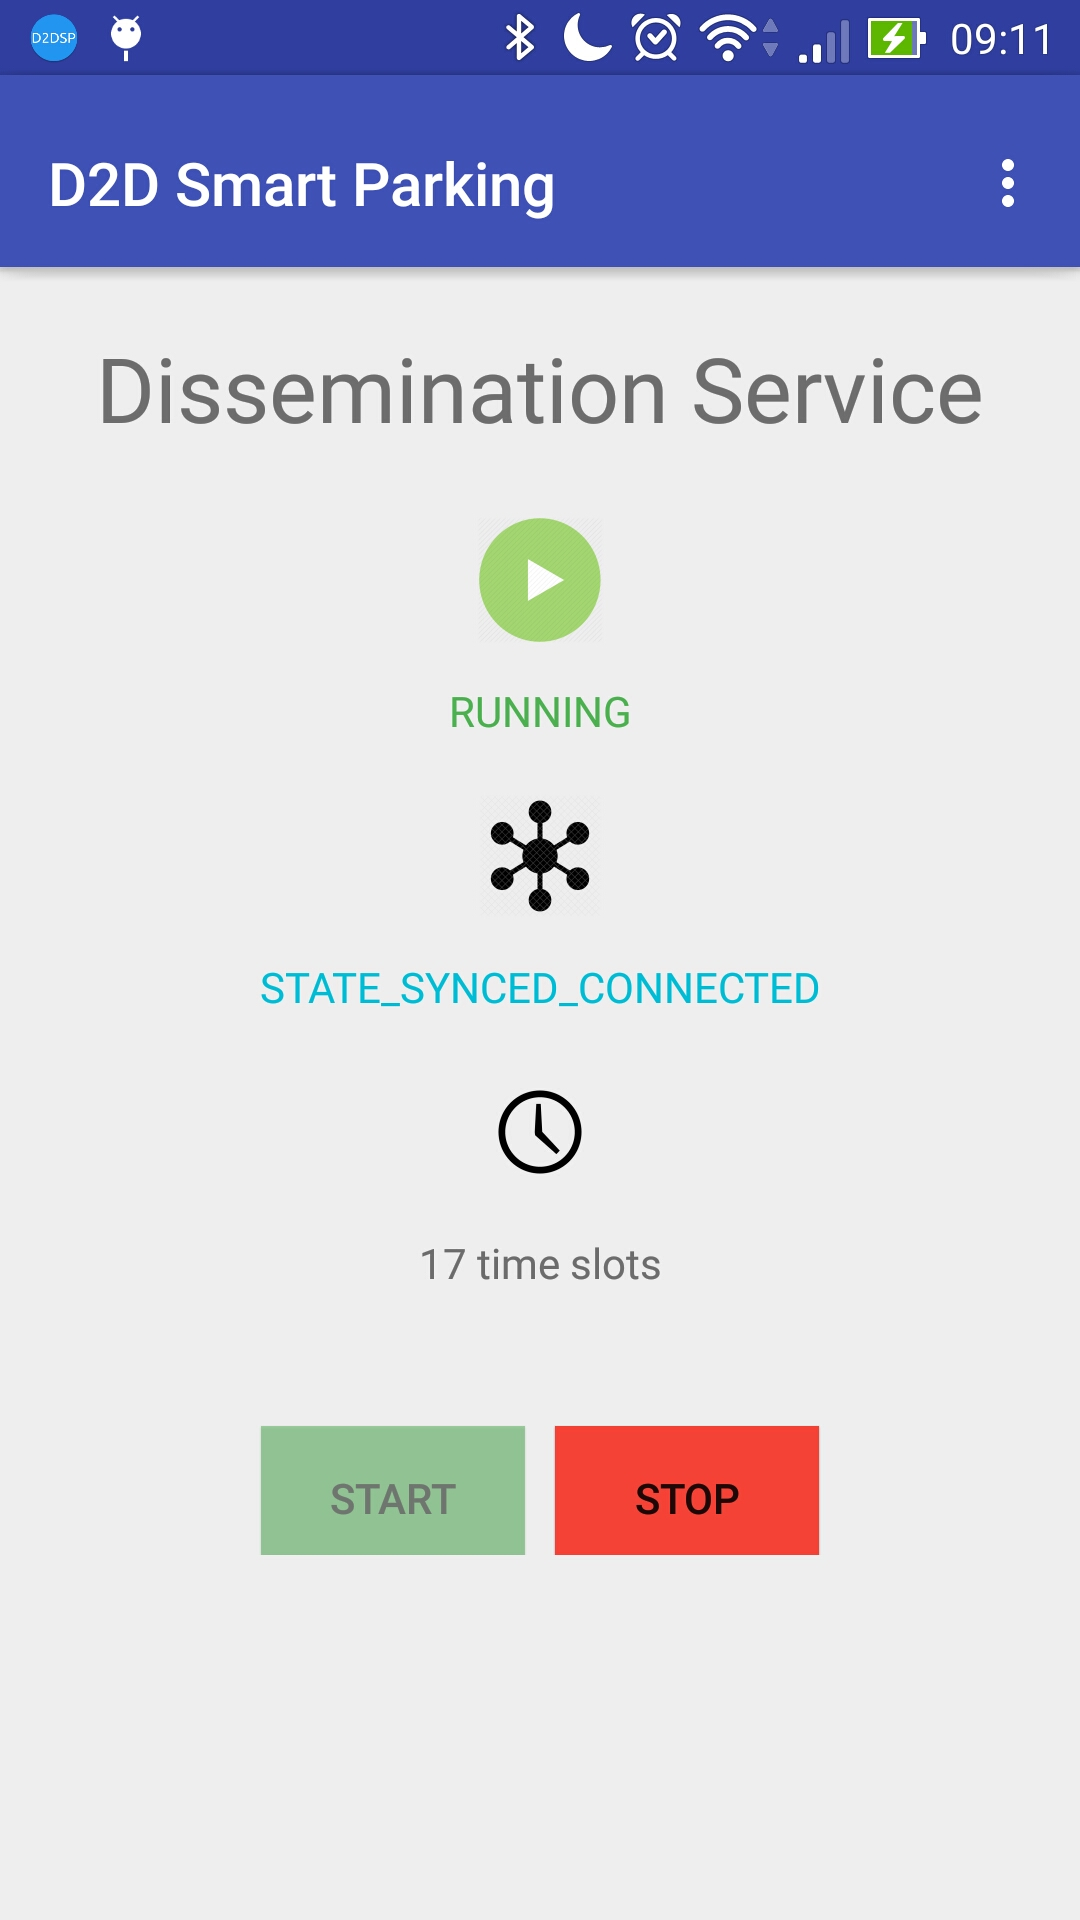
\includegraphics[width=\columnwidth]{img/screenshot/state_synced_connected.jpg}}
    \end{figure}
  \end{column}
  \begin{column}{0.25\textwidth}
    \begin{figure}
    \raggedleft
    \setlength{\fboxsep}{0pt}
    \setlength{\fboxrule}{0.1pt}
    \fcolorbox{blue}{blue}{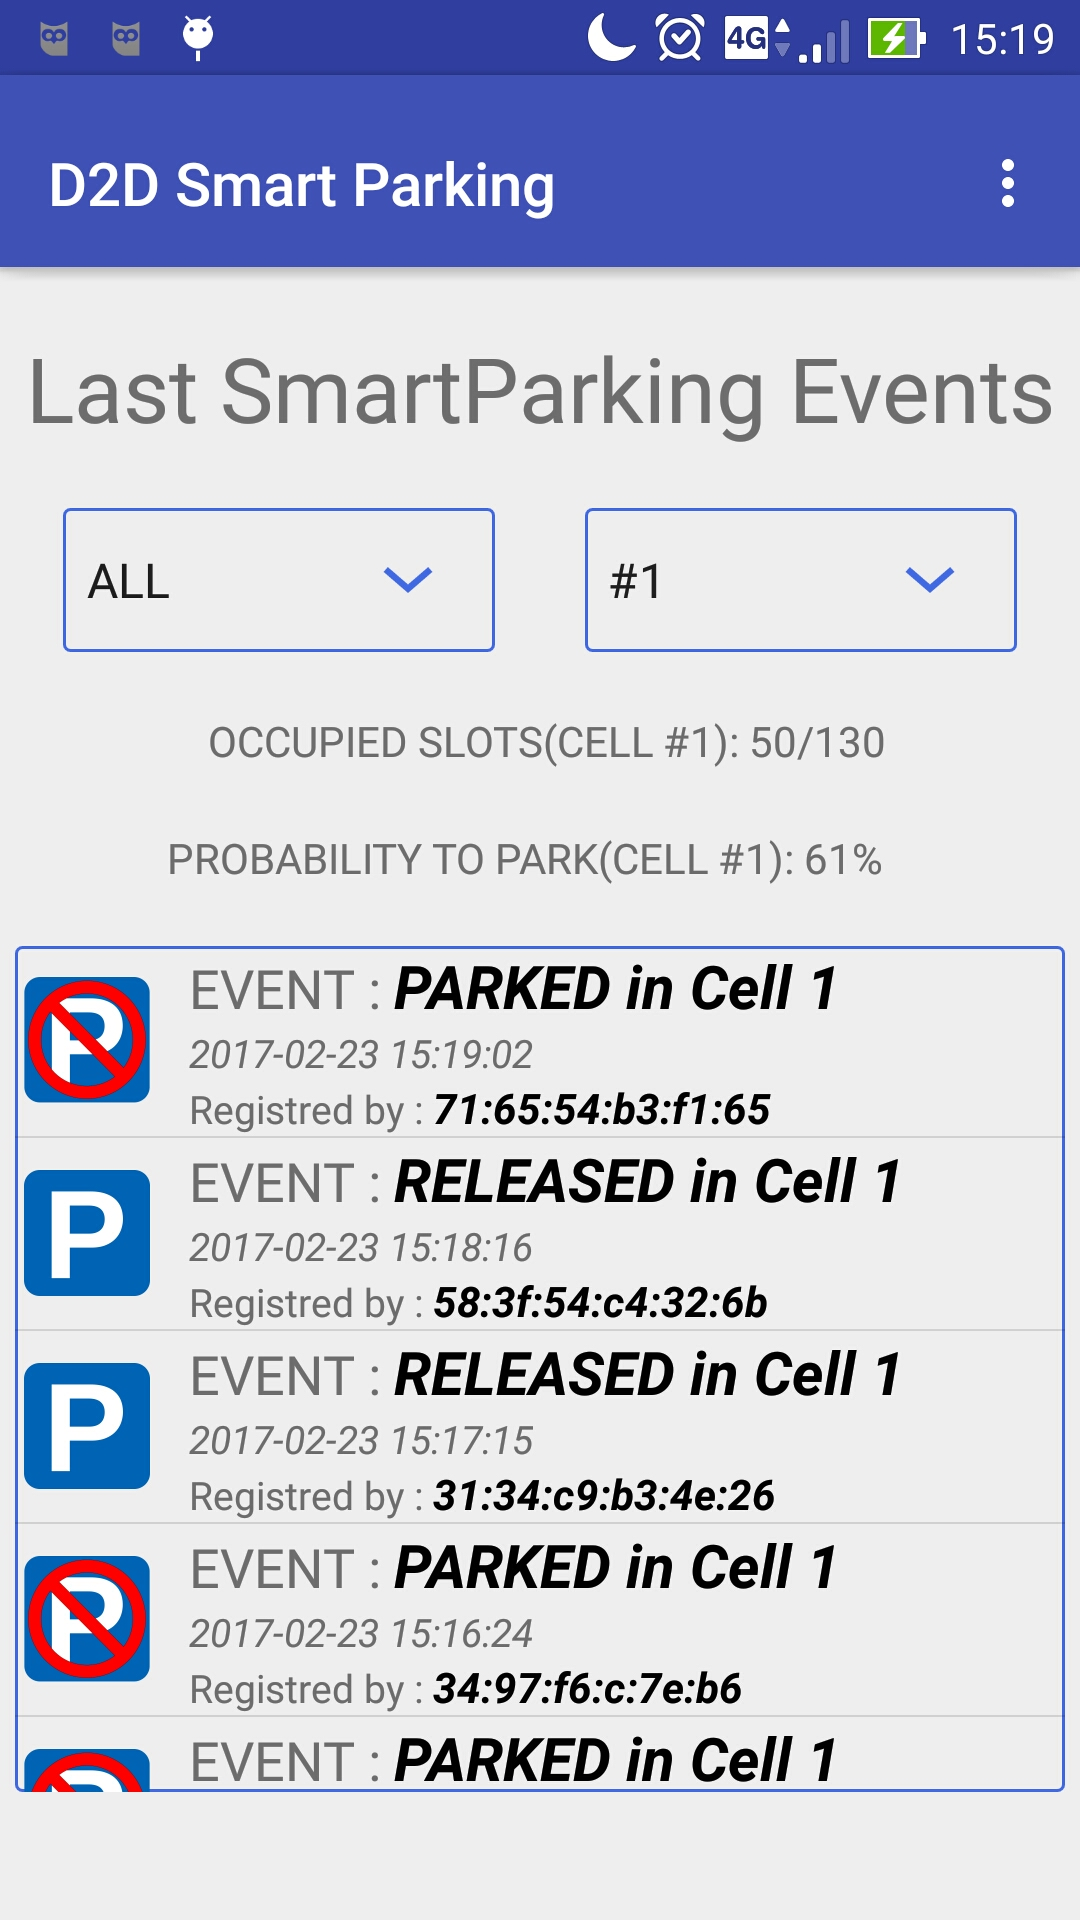
\includegraphics[width=\columnwidth]{img/screenshot/park_event_list.jpg}}
    \end{figure}
  \end{column}
  \begin{column}{0.25\textwidth}
    \begin{figure}
    \raggedleft
    \setlength{\fboxsep}{0pt}
    \setlength{\fboxrule}{0.1pt}
    \fcolorbox{blue}{blue}{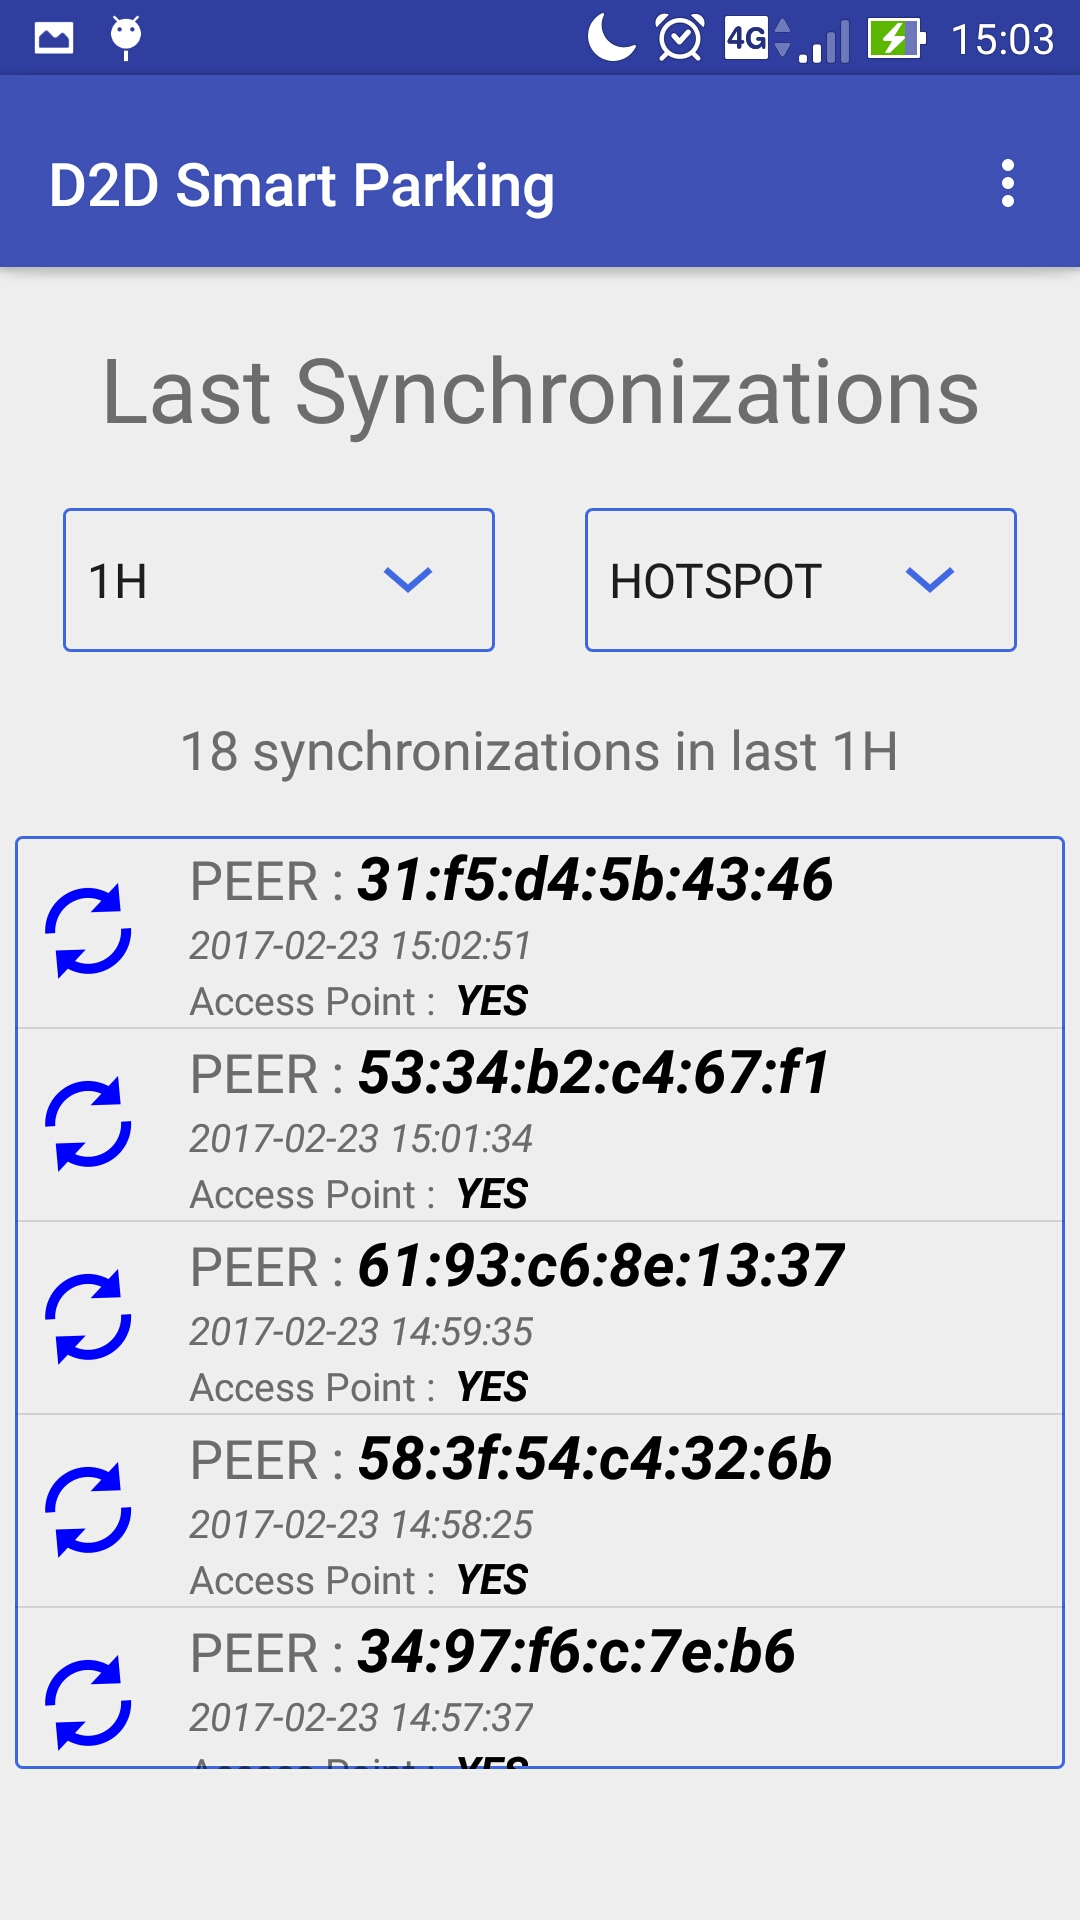
\includegraphics[width=\columnwidth]{img/screenshot/last_sync.jpg}}
    \end{figure}
  \end{column}
\end{columns}
\end{frame}


%------------------------------------------------

\begin{frame}
\frametitle{Bullet Points}
\begin{itemize}
\item Lorem ipsum dolor sit amet, consectetur adipiscing elit
\item Aliquam blandit faucibus nisi, sit amet dapibus enim tempus eu
\item Nulla commodo, erat quis gravida posuere, elit lacus lobortis est, quis porttitor odio mauris at libero
\item Nam cursus est eget velit posuere pellentesque
\item Vestibulum faucibus velit a augue condimentum quis convallis nulla gravida
\end{itemize}
\end{frame}

%------------------------------------------------

\begin{frame}
\frametitle{Blocks of Highlighted Text}
\begin{block}{Block 1}
Lorem ipsum dolor sit amet, consectetur adipiscing elit. Integer lectus nisl, ultricies in feugiat rutrum, porttitor sit amet augue. Aliquam ut tortor mauris. Sed volutpat ante purus, quis accumsan dolor.
\end{block}

\begin{block}{Block 2}
Pellentesque sed tellus purus. Class aptent taciti sociosqu ad litora torquent per conubia nostra, per inceptos himenaeos. Vestibulum quis magna at risus dictum tempor eu vitae velit.
\end{block}

\begin{block}{Block 3}
Suspendisse tincidunt sagittis gravida. Curabitur condimentum, enim sed venenatis rutrum, ipsum neque consectetur orci, sed blandit justo nisi ac lacus.
\end{block}
\end{frame}

%------------------------------------------------

\begin{frame}
\frametitle{Multiple Columns}
\begin{columns}[c] % The "c" option specifies centered vertical alignment while the "t" option is used for top vertical alignment

\column{.45\textwidth} % Left column and width
\textbf{Heading}
\begin{enumerate}
\item Statement
\item Explanation
\item Example
\end{enumerate}

\column{.5\textwidth} % Right column and width
Lorem ipsum dolor sit amet, consectetur adipiscing elit. Integer lectus nisl, ultricies in feugiat rutrum, porttitor sit amet augue. Aliquam ut tortor mauris. Sed volutpat ante purus, quis accumsan dolor.

\end{columns}
\end{frame}

\begin{frame}
\frametitle{Table}
\begin{table}
\begin{tabular}{l l l}
\toprule
\textbf{Treatments} & \textbf{Response 1} & \textbf{Response 2}\\
\midrule
Treatment 1 & 0.0003262 & 0.562 \\
Treatment 2 & 0.0015681 & 0.910 \\
Treatment 3 & 0.0009271 & 0.296 \\
\bottomrule
\end{tabular}
\caption{Table caption}
\end{table}
\end{frame}

%------------------------------------------------

\begin{frame}
\frametitle{Theorem}
\begin{theorem}[Mass--energy equivalence]
$E = mc^2$
\end{theorem}
\end{frame}

%------------------------------------------------

\begin{frame}[fragile] % Need to use the fragile option when verbatim is used in the slide
\frametitle{Verbatim}
\begin{example}[Theorem Slide Code]
\begin{verbatim}
\begin{frame}
\frametitle{Theorem}
\begin{theorem}[Mass--energy equivalence]
$E = mc^2$
\end{theorem}
\end{frame}\end{verbatim}
\end{example}
\end{frame}

%------------------------------------------------

\begin{frame}
\frametitle{Figure}
Uncomment the code on this slide to include your own image from the same directory as the template .TeX file.
%\begin{figure}
%\includegraphics[width=0.8\linewidth]{test}
%\end{figure}
\end{frame}

%------------------------------------------------

\begin{frame}[fragile] % Need to use the fragile option when verbatim is used in the slide
\frametitle{Citation}
An example of the \verb|\cite| command to cite within the presentation:\\~

This statement requires citation \cite{p1}.
\end{frame}

%------------------------------------------------

\begin{frame}
\frametitle{References}
\footnotesize{
\begin{thebibliography}{99} % Beamer does not support BibTeX so references must be inserted manually as below
\bibitem[Smith, 2012]{p1} John Smith (2012)
\newblock Title of the publication
\newblock \emph{Journal Name} 12(3), 45 -- 678.
\end{thebibliography}
}
\end{frame}

%------------------------------------------------

\begin{frame}
\Huge{\centerline{Grazie per l'attenzione!}}
\end{frame}

%----------------------------------------------------------------------------------------

\end{document}